\documentclass{acmsiggraph}               % final
%\documentclass[review]{acmsiggraph}      % review
%\documentclass[widereview]{acmsiggraph}  % wide-spaced review
%\documentclass[preprint]{acmsiggraph}    % preprint
%\preprinttext{Confidential draft - do not distribute. Date: 2005-07-27}

%% Uncomment one of the four lines above depending on where your paper is
%% in the conference process. ``review'' and ``widereview'' are for review
%% submission, ``preprint'' is for pre-publication, and ``final'' is for
%% the version to be printed.

%% These two line bring in essential packages: ``mathptmx'' for Type 1
%% typefaces, and ``graphicx'' for inclusion of EPS figures.

\newif\ifpdf
\ifx\pdfoutput\undefined
   \pdffalse      % we are not running PDFLaTeX
\else
   \pdfoutput=1   % we are running PDFLaTeX
   \pdftrue
\fi

\usepackage{amsmath}                    % Typical maths resource packages
\usepackage{amsfonts}                   % if you want the fonts
\usepackage{amssymb}                    % if you want extra symbols
\usepackage{amsthm}

\usepackage{mathptmx}
\usepackage{graphicx}
\usepackage{amsmath}
\usepackage{url}


\acmcategory{Research}
\acmformat{print}

%% Paper title.

\title{M3G Project in EDA075 Mobile Computer Graphics}

%% Author / Affiliation (single author).

%%\author{Roy G. Biv}
%%\affiliation{Allied Widgets Research\thanks{email:roy.g.biv@aol.com}}

%% Author / Affiliation (multiple authors).

\author{Magnus Borg\thanks{e-mail: d02mbo@efd.lth.se} \and Erik Zivkovic\thanks{e-mail: d02ez@efd.lth.se}
}
\affiliation{Lund University\\ Sweden}


%% Keywords that describe your work.
\keywords{M3G Game}

%%%%%% START OF THE PAPER %%%%%%

\begin{document}

\ifpdf
  \DeclareGraphicsExtensions{.jpg,.pdf,.mps,.png}
\else
  \DeclareGraphicsExtensions{.eps}
\fi


\maketitle

\begin{abstract}
The abilities of today's mobile platforms are getting closer to the specifications
of modern desktopplatforms, according to multimedia capabilities, such as special
GPUs and faster memory, but also at the same time introducing different kinds of 
input, for example video cameras, accelerometers and GPS. There are also different 
kinds of packages that manage 3d applications, one of those packages is M3G.

In this paper, we describe the development of a game for mobile phones
using the mentioned M3G package. This paper and the developed software are part 
of a project in the course EDA075 Mobile Computer Graphics at
the Department of Computer Science, Lund University. 
\end{abstract}


\section{Introduction}
In this paper we will describe the whole development process for the game, but we
will review certain points of interest, such as design, architecture and 3d-modeling.
The guidelines for the M3G project weren't strict, but two students are supposed to
work on the project for 2 weeks, per student. 
We chose to design and implement a game using the M3G package and we had different 
ideas but settled for a lowrider game. A lowrider is a car that uses controllable 
hydraulics instead of suspension. The whole concept was born in California in the 
early '60s, when a car got equipped with a pump and hydraulics from a B-52 bomber
\footnote{An american fighting airplane}.
Today there are contest where the competitor tries to jump as high as possible by
using the hydraulics. 
In this game we wanted to mimic these cars and their abilities by using the M3G 
package.  


\section{Application}

\subsection{Design}
First we needed a basic idea for the game and the different modes. We wanted the
user to be able to play by himself, but also be able to enjoy the competition of
a friend in a multiplayer game.
We also needed different type of game modes, and we chose to implement three different
gaming modes. To further extend the longevity of the game we also wanted to include 
a memory based highscore.
\\
These are the available game modes:
\begin{itemize}
    \item Singleplayer
    	\begin{itemize}
    		\item High hop - get the car to jump as high as possible.
    		\item Car dance -  get the car to do certain dance moves. 
    		\item Training - get the car to jump.
    	\end{itemize}
    \item Multiplayer
    	\begin{itemize}
    		\item High hop - get the car to jump as high as possible.
    		\item Car dance -  get the car to do certain dance moves. 
    	\end{itemize}
\end{itemize}

We wanted the player to get into the right feeling, and to further enhance the feel of 
the game we introduced special background images, a theme song, different environments
and different cars.
\\\\
These are the available environments: 
\begin{itemize}
    \item USA - Los Angeles - A backalley in Compton.
    \item Sweden - Lund - A parkinglot at Delphi.
\end{itemize}    
These are the available cars: 
\begin{itemize}
    \item Cheverolet - 1964 - Impala
    \item Cheverolet - 1978 - Monte Carlo
    \item Volvo - 1992 - 240
\end{itemize}    

\subsection{Architecture}
To save the limited amounts of memory and computing power on the phone, we needed to invent a strategy 
that could load everything we wanted and at the same time give visual output while we were doing it. It 
proved to be an non-trivial task. First of all, we knew we had to limit the amount of threads running in 
the system. We actually only have two:
\begin{itemize}
    \item LWRRenderThread - the thread in charge of the refresh rate.
    \item LWRSplash - the thread in charge of loading the next scene.
\end{itemize}

The class LWRMain which contains the starting point for the project actually also has Thread-like qualities 
(it registers a CommandListener which distributes commands into the monitor). But we have chosen not to include 
it in the list of Threads, since we are not in charge of what it does, or how it does it.
\\\\
We have abstracted all the different scenes, menus and splash-screens into something we call an LWRAbstractGame. 
This way we can force every class to obey certain rules, for instance every type of scene renders in the same way 
which lets us use the same logic for rendering all the different types of scenes. 
\\\\
One obstacle we faced when implementing the switch between e.g. menu and scene was that we ran out of memory on the phone. 
We solved this by using a middle-man, called LWRSplash. LWRSplash first loads a splash screen, then exits the constructor. 
The calling method then calls flush (sets everything to null and calls gc) on itself, and when that is done it starts the 
splash screen thread which loads the next environment or menu.
\\\\
We call the central middle-man in our project LWRMonitor. This is misleading, because its about as minimal 
as a monitor can get. It only holds the currently rendering LWRAbstractGame, forces it to repaint and forwards 
system calls (key presses) to it.


\subsection{3d-Modeling}
By using external 3d-modeling application we managed to create realistic environments
and lifelike cars. The entire process of making a fully textured model is greately 
quickend by this. We chose to use LightWave as a modeling tool and HI Corps h3t exporter.
The models mainly use UV-texturing, and map sizes range from 32x32 to 128x128 pixels.
All models are made from reference pictures from the internet. 
For simple shadow support we added a single black quad polygon with transperancy 
under the modeled cars. 

\section{Results}

The use of high level abstractions and the use of middle-man classes turned out to be a winning concept. We have 
reasonable loading times, acceptable performance and a skeleton that is easy to expand (which we have proven with 
our different game types, cars and levels). 
As far as graphical content we think we have managed to present a nice looking 3D-game, and a interesting 
atmosphere. We have included som screen captures from the game run in the emulator.

\begin{figure}[tb]
    \centering
    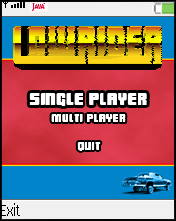
\includegraphics[width=0.6\columnwidth]{bild1-meny.png}
    \caption{Screenshot of the menu system}
    \label{fig_bild1}
\end{figure}

\begin{figure}[tb]
    \centering
    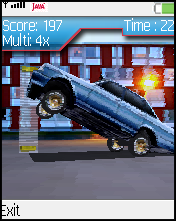
\includegraphics[width=0.6\columnwidth]{bild2-cardance.png}
    \caption{Screenshot of the high hop mode(Volvo 240)}
    \label{fig_bild2}
\end{figure}

\section{Discussion}

\subsection{Media Issues}
The performance on the actual mobile phones is greatly affected by the memory use.
To minimize the memory resources needed, we experimented with different sizes and 
formats for the images files that are used in the game. The PNG fileformat is used
for all the images. The maximum allowed dimension for images in M3G are 256x256 pixels 
which is more then enough for smaller displays, but this is supposed to change in 
future M3G versions. We made our textures at most 128x128 pixels in size. There are 
also different PNG formats, 32 , 24 or 8 bits. 32 bits is way over the top for todays
phones, and the 24 bits format still have a alpha channel, which the 8 bit format lacks. 
We chose an optimized 24 bit format. At first we had almost 1.3 Mb loaded at an 
in-game state, and after we resized and optimized all the images (sprites, backgrounds
and textures) and compressed the M3G format we ended up with only using 0.3 Mb of memory at an 
in-game state.

The audio files that are used are in MP3 format with a low bitrate to reduce size. We
also encountered problems while playing multiple sounds. I.e. playing multiple sounds simultaneously.

In-game we use a MP3 file for sound effects and iMelody files to control the vibrator
in the mobilephone.

\subsection{Memory Issues}
We did most of our testing on a Sony Ericsson V800 (Z800). This mobile phone has
a heap size of 512 Kb and can expand dynamically to approximately 1500 Kb. We had
problems during loading (using MP3 audio, background images, M3G scenes and sprites)
After optimizing the media and shortening the audio we managed to get the game running.
It is also recommended to release memory at controlled moments, by implementing a
flush method we release objects and then call the garbage collector, and by doing this
we ensure the functionality of the application and also reduce lag during different
stages in the game.


\bibliographystyle{acmsiggraph}
%\nocite{*}
\bibliography{project}
\end{document}